\section{Performance Analysis}
\label{sec:perfanalysis}
In our tool we have developer a \textit{script} which records timestamps and duration time of big data analysis in a \texttt{.csv} file, called \texttt{PerformanceHistory.csv}. The \textit{script} mentioned before is used in order to figure out the time of analysis. 
The environment in which we tested our tool is a cluster of the University of Verona, running Ubuntu 18.04.1 LTS, it has an Intel Xeon Processor Skylake (4 cores @ 2,6 GHz) and a RAM memory of 7880 MiB for a single node, in its total configuration it has ten VCore and 60GB of RAM memory. 
We have never observed a total usage of more of 10\% CPU using \texttt{top} command and, in general, memory usage is often below 3000 MiB.
 
Using our script called \texttt{PerformanceAnalysis.py} we managed to plot the time elapsed to analyse the datasets listed into Tab. \ref{tab:dataset_info}: results are reported into Fig. \ref{fig:analysis_stats}. 

\begin{figure}[ht]
	\centering
	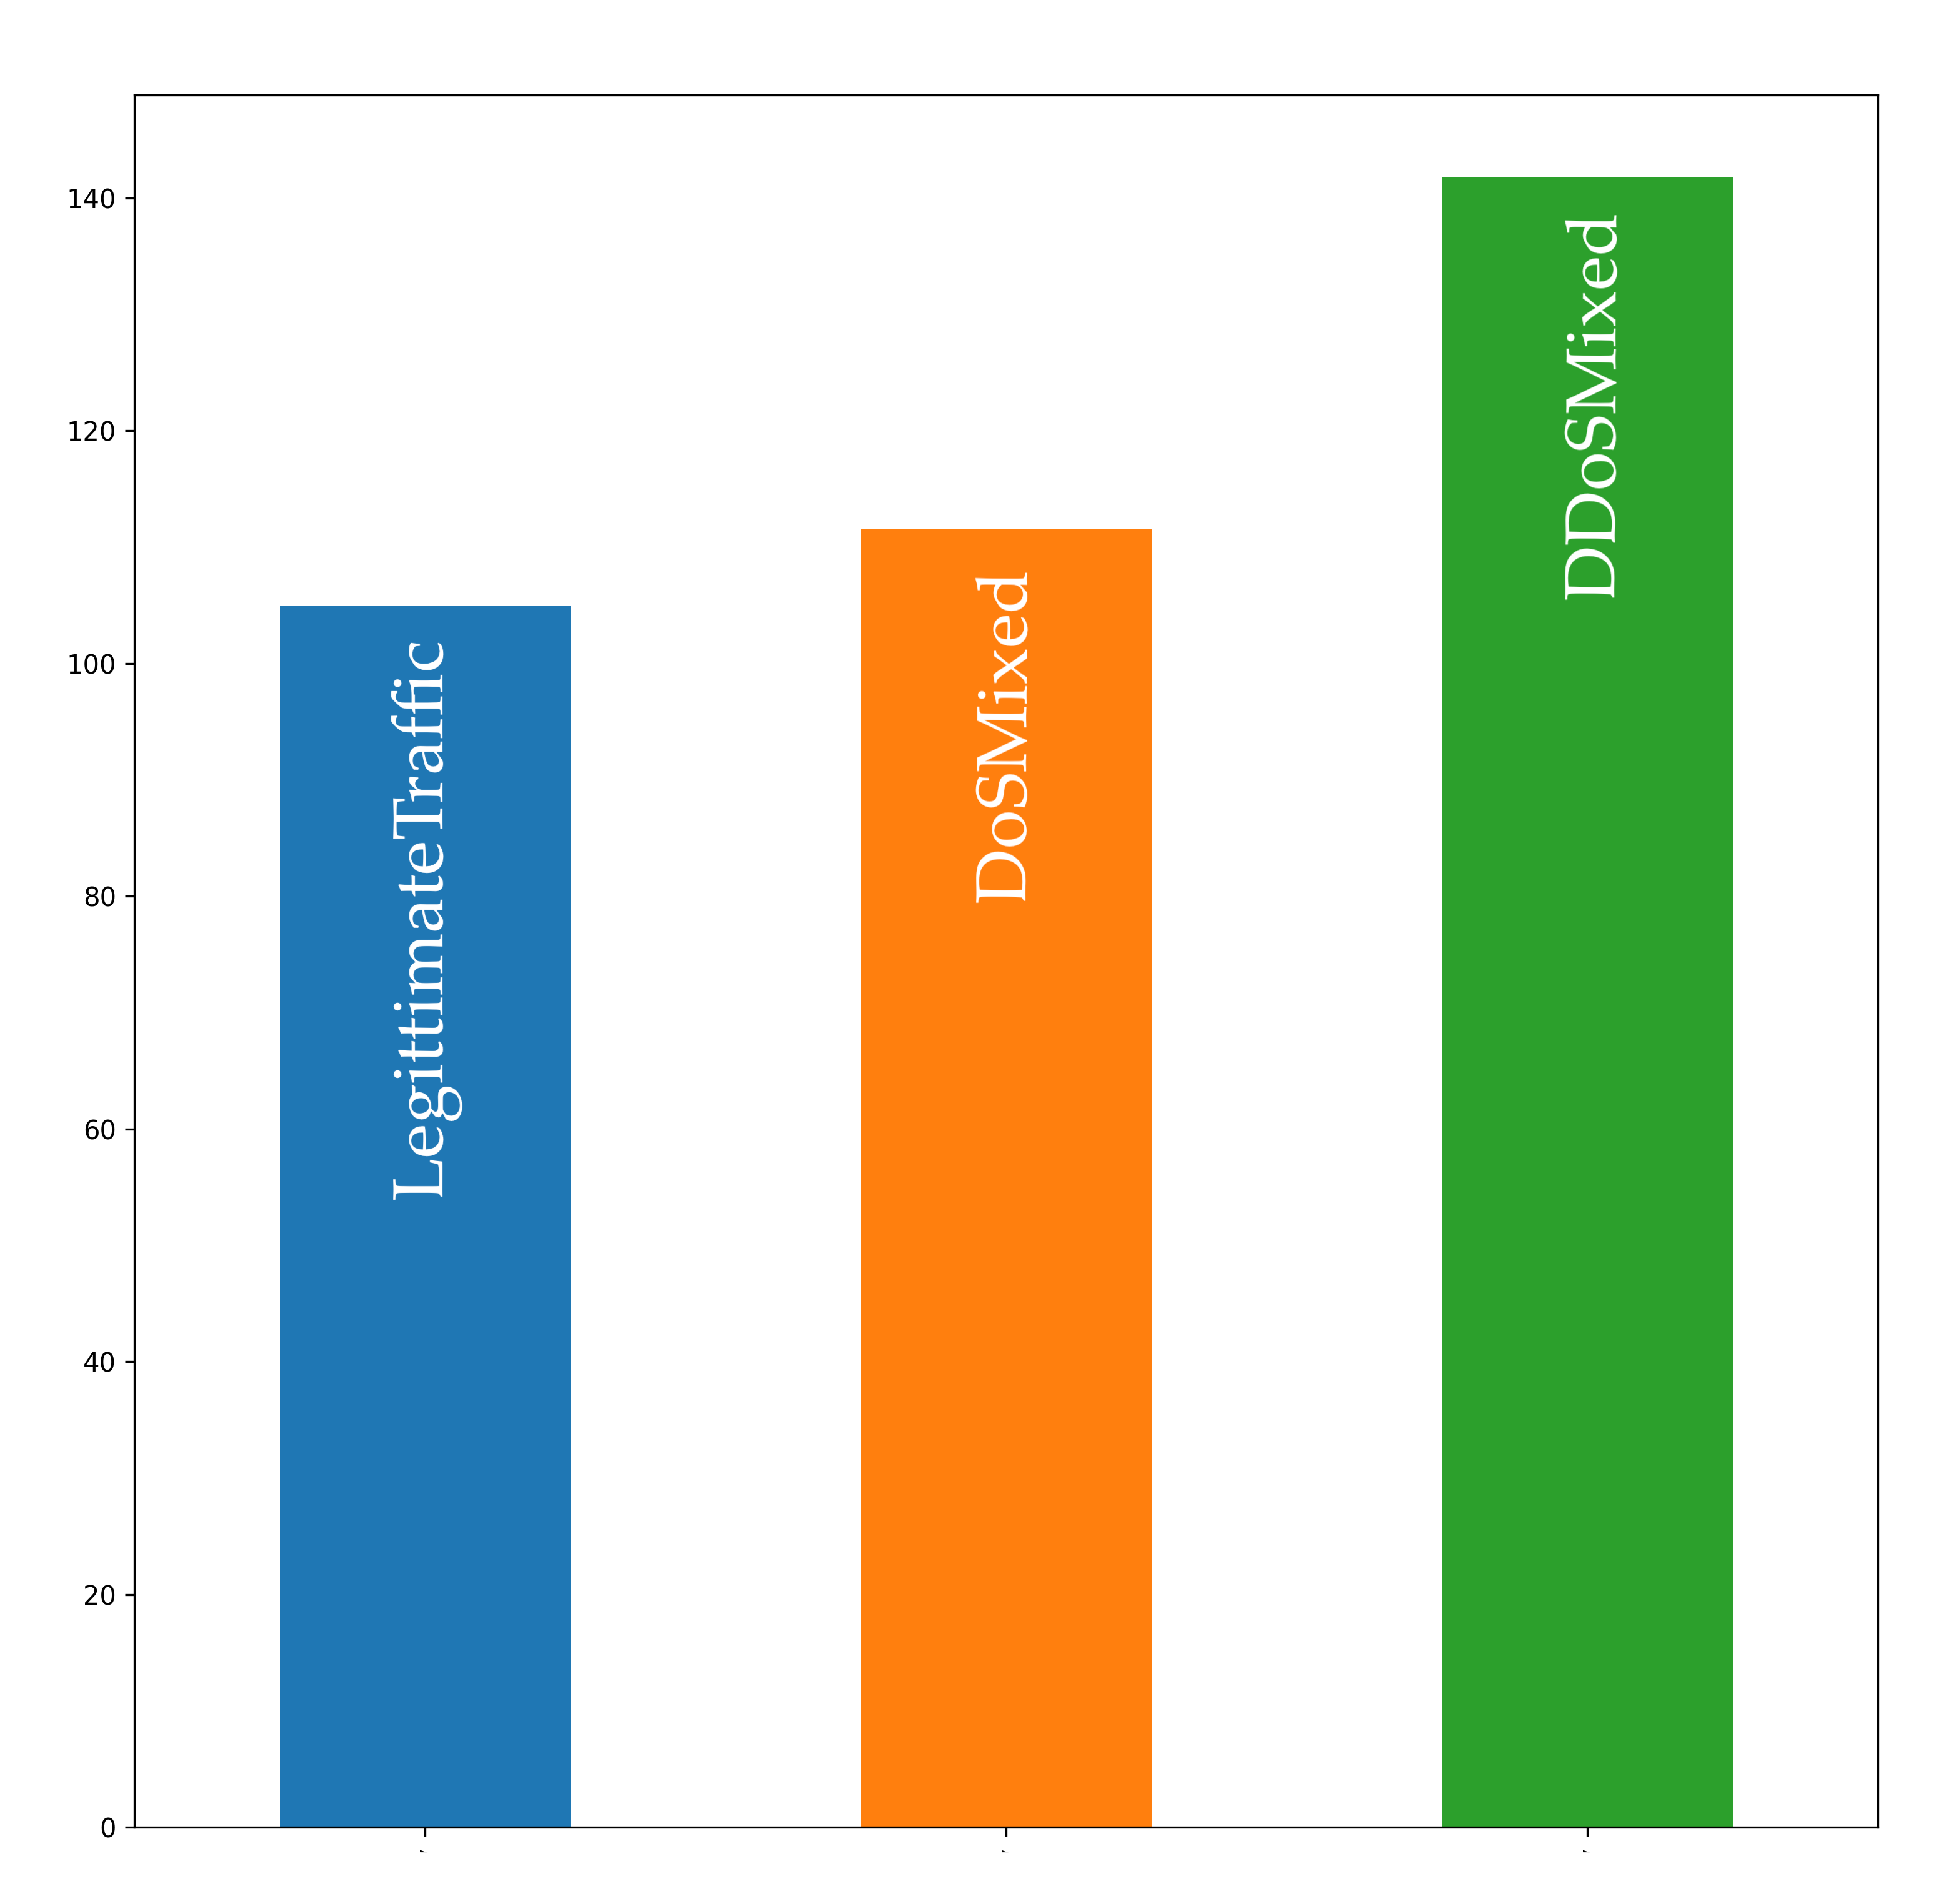
\includegraphics[scale=0.25]{imgs/analysis_stat.png}
	\caption{Performance Analysis} 
	\label{fig:analysis_stats}
\end{figure}
In \textbf{Tab. \ref{tab:dataset_info}} we show a summary of the dimension of the datasets we have used in our analysis. Both the \textit{LegitimateTraffic} and \textit{DoSMixed} datasets were completed in approximately 1 minute and 40 seconds. \textit{DDoSMixed} was completed in 2 minutes and 17 seconds, but it's not a noticeable increment, considering the fact that it's way bigger. This justifies the parallel approach we have used with \textbf{Pig Latin}.

\begin{table}[!htbp]
\centering
\begin{tabular}{|l|l|c|}
\hline
\textbf{Dataset} & \textbf{Description}                              & \textbf{Size} \\ \hline
LegitimateTraffic         & Traffic log in normal conditions. & 316 KB        \\ 
DoSMixed        & Traffic log during a DoS attack.                   & 89 MB       \\ 
DDoSMixed        & Traffic log during a DDoS attack. & 612 MB        \\ \hline
\end{tabular}
\caption{Datasets Info}
\label{tab:dataset_info}
\end{table}

Looking at our job stats, we have noticed that for the \textit{LegitimateTraffic} the average reduce time is zero, and for the other two datasets the average map time exceeds the reduce one.

